\chapter{Background} \label{ch:background} Areas of artificial intelligence deal with autonomous planning or deliberation for robotic systems to navigate through an environment. A detailed understanding of these environments is required to navigate through them. High-level information about the environment could be provided by a computer vision system that is acting as a vision sensor.

In this thesis, we will focus on building hand gesture recognition system for a humanoid robot name as NAO, with the help of computer vision algorithms to track the skeletal points of human body using depth camera. Following sections clearly studies the key concepts of this thesis.

\section{NAO - The Humanoid Robot} NAO is an autonomous programmable humanoid robot invented by Aldebaran Robotics. NAO Academics Edition is developed for universities and laboratories for research and educational purposes. Follow subsections discuss briefly about the specifications of NAO as described by Aldebaran Robotics \cite{8}.

\begin{table}
	[h] \centering \caption{NAO V5 specification } \label{tb:nao:spec} 
	\begin{tabular}
		{|l|l|} \hline Height & 58 centimetres (23 in) \\
		\hline Weight & 4.3 kilograms (9.5 lb) \\
		\hline Battery autonomy & 60 minutes (active use), 90 minutes (normal use) \\
		\hline Degrees of freedom & 21 to 25 \\
		\hline CPU & Intel Atom @ 1.6 GHz \\
		\hline Built-in OS & Linux \\
		\hline SDK compatibility & Windows, Mac OS, Linux \\
		\hline Programming languages & C++, Python, Java, MATLAB, Urbi, C, .Net \\
		\hline Vision & 2 x HD 1280x960 cameras \\
		\hline Connectivity & Ethernet, Wi-Fi \\
		\hline \multirow{6}{*}{Sensors} & 4 x directional microphones \\
		& 1 x sonar rangefinder \\
		& 2 x IR emitters and receivers \\
		& 1 x inertial board \\
		& 9 x tactile sensors \\
		& 8 x pressure sensors \\
		\hline 
	\end{tabular}
\end{table}


\subsection{Body} NAO has a body with 25 degrees of freedom (DOF) whose key elements are electric motors and actuators as show in the figure \ref{fg:nao:body}. It has 48.6-watt-hour battery that provides 1.5 or more hours of autonomy, depending on the usage. Additional specifications of robot are shown in the table \ref{tb:nao:spec}. 

\begin{figure}
	\begin{minipage}
		{.6
			\textwidth} 
		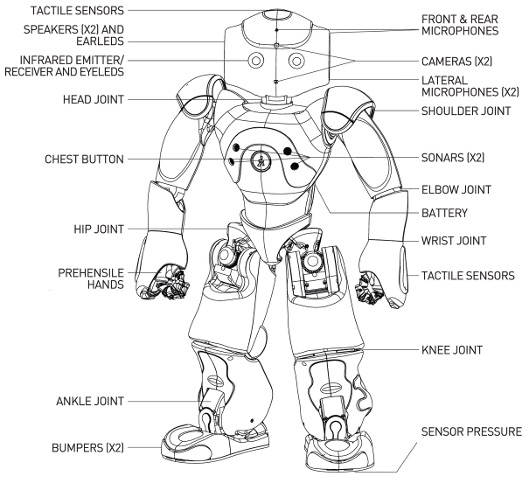
\includegraphics[height=7cm]{figures/content/nao-body.jpg} 
	\end{minipage}
	\begin{minipage}
		{.4 
			\textwidth} 
		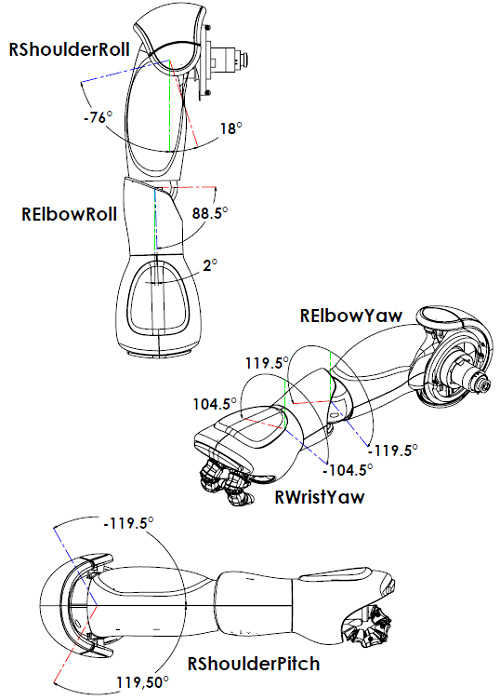
\includegraphics[height=7cm]{figures/content/nao-hand.jpg} 
	\end{minipage}
	\begin{minipage}
		{.6 
			\textwidth} 
		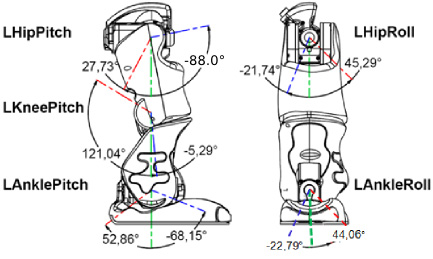
\includegraphics[height=50mm]{figures/content/nao-leg.jpg} 
	\end{minipage}
	\begin{minipage}
		{.4 
			\textwidth} 
		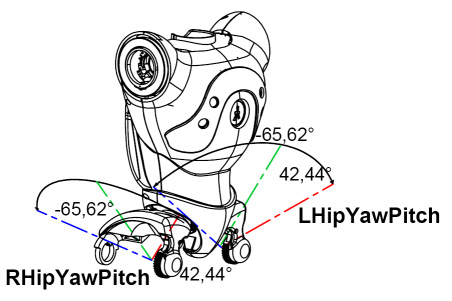
\includegraphics[height=40mm]{figures/content/nao-hip.jpg} 
	\end{minipage}
	\caption{Shoulder, Leg and Hip joints illustrating the body construction of NAO V5 \cite{nao-spec}} \label{fg:nao:body} 
\end{figure}


\subsection{Motion} NAOs walking algorithm uses a simple dynamic model (linear inverse pendulum) and quadratic programming. It is stabilized using feedback from the joint sensors. This makes the walking robust and resistant to small disturbances, and torso oscillations in the frontal and lateral planes are absorbed. It can walk on a variety of floor surfaces, such as carpeted, tiled, and wooden floors. 

NAOs motion module is based on generalized inverse kinematics, which handles locomotion, joint control, balance, redundancy, and task priority. This means that when asking it to extend its arm, it bends over because its arms and leg joints are taken into account.

\begin{figure}
	\centering 
	\begin{minipage}
		{.3 
		\textwidth} \centering 
		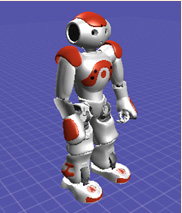
\includegraphics[height=5cm]{/content/nao-stand.jpg} 
	\end{minipage}
	\begin{minipage}
		{.3 
		\textwidth} \centering 
		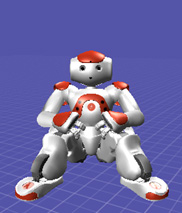
\includegraphics[height=5cm]{/content/nao-sit.jpg} 
	\end{minipage}
	\begin{minipage}
		{.3 
		\textwidth} \centering 
		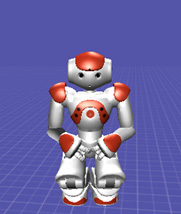
\includegraphics[height=5cm]{/content/nao-crouch.jpg} 
	\end{minipage}
	\caption{Standing, Sitting and Crouching postures of virtual NAO using ALRobotPosture module. \cite{8}} \label{fg:nao:motion} 
\end{figure}


In this thesis, we attempt to use the locomotion and stiffness control of Motion API to move NAO to a position in the two dimensional space. Robot Posture API will also be used to make the robot go to the predefined posture such as Stand, Sit and Crouch as shown in the figure \ref{fg:nao:motion}. Python code \ref{code:nao:motion} shows how the robot can be moved to another position at the given normalized velocity using Motion API. 

\lstinputlisting[language=python]{code/nao-motion.py} \label{code:nao:motion}

\subsection{Audio} NAO uses four directional microphones to detect sounds and equipped with a stereo broadcast system made up of 2 loudspeakers in its ears as shown in the figure \ref{fg:nao:audio}. NAOs voice recognition and text-to-speech capabilities allow it to communicate in 19 languages. 

\begin{figure}
	[h] \centering 
	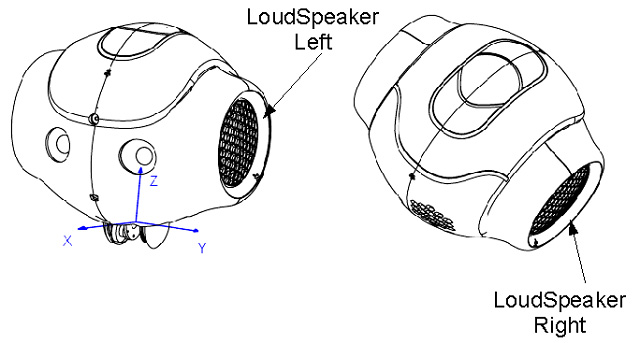
\includegraphics[height=7cm]{figures/content/nao-audio.jpg} \caption{NAO Audio} \label{fg:nao:audio} 
\end{figure}
 

In this thesis, we aim to use Text-To-Speech API of NAO to say the detected gesture loud to communicate with the user. Python code \ref{code:nao:audio} shows how NAO can say words given as strings.

\lstinputlisting[language=python]{code/nao-audio.py} \label{code:nao:audio}

\begin{figure}
	[h] \centering 
	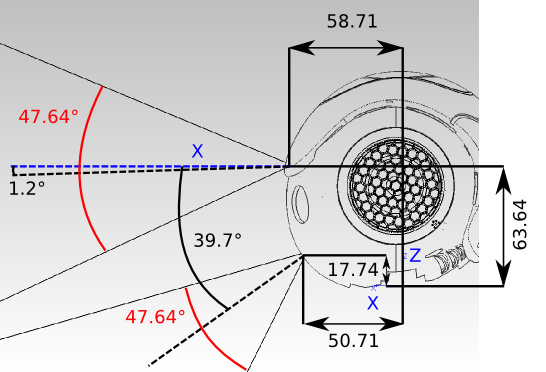
\includegraphics[height=7cm]{figures/content/nao-vision.jpg} \caption{The field of view of two identical RGB video cameras which are located in the forehead of NAO. \cite{8} } \label{fg:nao:vision} 
\end{figure}


\subsection{Vision} \label{sec:nao:vision} Proper vision is the utmost importance for the function of any vision based autonomous robot. Areas of artificial intelligence deal with autonomous planning or deliberation for robotic systems to navigate through an environment. High-level information about the environment could be provided by a computer vision system that is acting as a vision of the robot.

Two identical video RGB cameras are located in the forehead of NAO as shown in the figure \ref{fg:nao:vision}. They provide up to 1280x960 resolution at 30 frames per second. Aldebaran provides a set of algorithms for detecting and recognizing faces and shapes.

\paragraph*{Depth Image} Skeletal points based gesture recognition needs three dimensional data of the human skeleton. However, sensors integrated with NAO could not provide precise three dimensional data to the sophisticated algorithms to track human skeletal joints. 3D cameras such as Microsoft Kinect and Asus Xtion are used not only for gaming but also for analyzing 3D data, including algorithms for feature selection, scene analysis, motion tracking, skeletal tracking and gesture recognition \cite{9}. Therefore, we seek to utilize Asus Xtion PRO LIVE as an external camera to support the skeletal points tracking system of NAO. 

\begin{figure}
	[h] \centering 
	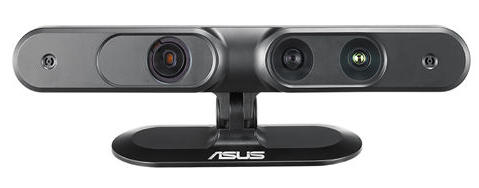
\includegraphics[height=4cm]{figures/content/xtion.png} 
	\caption{Asus Xtion Pro Live}
	\label{fg:xtion} 
\end{figure}

\paragraph*{Asus Xtion} Figure \ref{fg:xtion} shows Asus Xtion PRO LIVE that uses infrared sensors, adaptive depth detection technology, color image sensing and audio stream to capture a 3D image of the user in real-time. It uses infrared emitters to project speckle patterns on the object and uses a structured light technique to compute the depth of the image. Once the depth image is computed, it is mapped onto the RGB image as shown in the figure \ref{fg:xtion:depth}. Lighter color denote that a pixel is closer to the camera and darker color denotes that a pixel is far from the camera.

\begin{figure}
	[h] \centering 
	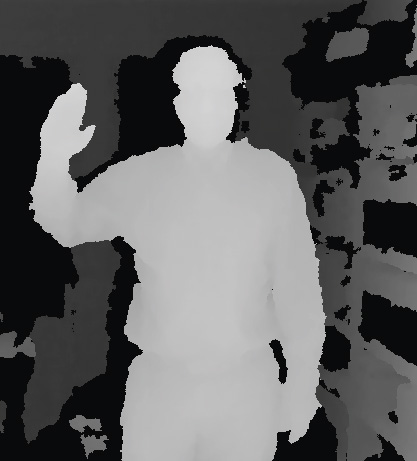
\includegraphics[height=8cm]{figures/content/xtion-depth.jpg} 	
	\caption{Depth Image recorded by depth camera Asus Xtion Pro Live} \label{fg:xtion:depth} 
\end{figure}


\subsection{Computing} NAO is equipped with Intel ATOM 1.6 GHz CPU in the head that runs a 32 bit Gentoo Linux to support Aldebarans proprietary middleware (NAOqi). NAOqi SDK is the programming framework used to program Aldebaran robots \cite{8}. This framework allows homogeneous communication between different modules such as motion, audio and video. NAOqi executable that runs on the robot is a broker. The broker provides lookup services so that any module in the tree or across the network can find any method that has been advertised as shown in the figure \ref{fg:nao:proxy}.

\begin{figure}
	[h] \centering 
	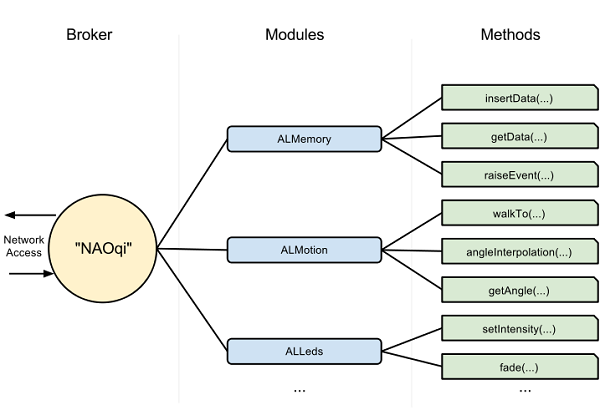
\includegraphics[height=7cm]{figures/content/nao-proxy.png} 
	\caption{NAOqi Proxy}
	\label{fg:nao:proxy} 
\end{figure}

Computational limitations of NAOs CPU hinders us to build a real time gesture recognition based on human skeletal joints. Thus, we aim to use an off-board computer to execute the gesture recognition program and communicated with NAO via NAOqi proxies. 
 
\section{Gesture Recognition} Human hand gestures are a means of nonverbal interaction among people. They range from simple actions of using our hand to point at, to the more complex ones that express our feelings and allow us to communicate with others. To exploit the use of gestures in HRI, it is necessary to provide the means by which they can be interpreted by robots. The HRI interpretation of gestures requires that dynamic and/or static configurations of the human hand, arm and even other parts of the human body, be measurable by the machine \cite{6}. 

Initial attempts to recognize hand gestures resulted in electro-mechanical devices that directly measure hand and/or arm joint angles and spatial position using sensors \cite{3}. Glove-based gestural interfaces require the user to wear such a complex device that hinders the ease and naturalness with which the user can interact with the computer controlled environment. 

Even though such hand gloves are used in highly specialized domain such as simulation of medical surgery or even in the real surgery, the everyday user will be certainly deterred by such sophisticated interfacing devices. As an active result of the motivated research in HRI, computer vision based techniques were innovated to augment the naturalness of interaction.

\subsection{Gesture Modeling} Figure \ref{fg:ges:model} shows various types of modeling techniques used for Gesture modeling \cite{3}. Selection of an appropriate gesture modeling depends primarily on the intended application. For an application that needs just hand gesture to go up and down or left and light, a very simple model may be sufficient. However, if the purpose is a natural-like interaction, a model has to be sophisticated enough to interpret all the possible gesture. The following section discusses various gesture modeling techniques which are being used by the existing hand gesture recognition applications. 

\begin{figure}
	[h] \centering 
	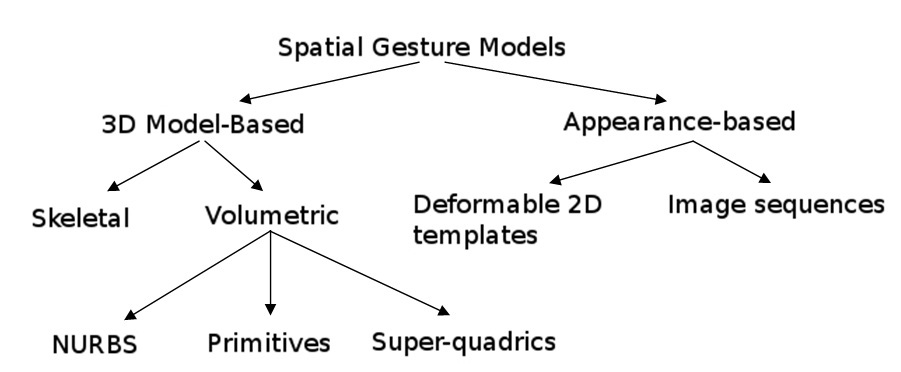
\includegraphics[width=130mm]{figures/content/ges-model.jpg} \caption{Types of Spatial Gesture Modeling. \cite{2}} \label{fg:ges:model} 
\end{figure}


Appearance based models don't use the spatial representation of the body, because they derive the parameters directly from the images or videos using a template database. Volumetric approaches have been heavily used in computer animation industry and for computer vision purposes. The models are generally created of complicated 3D surfaces. The drawback of this method is that is very computational intensive. 

Instead of using intensive processing of 3D hand models and dealing with a lot of parameters, one can just use a simplified version that analyses the joint angle parameters along with segment length. This is known as a skeletal representation of the body, where a virtual skeleton of the person is computed and parts of the body are mapped to certain segments \cite{4}. The analysis here is done using the position and orientation of these segments or the relation between each one of them.

In this thesis, we focus on skeletal based modeling, that is faster because the recognition program has to focus only on the significant parts of the body.

\subsection{Gestural Taxonomy} Several alternative taxonomies have been suggested that deal with psychological aspects of gestures \cite{3}. All hand/arm movements are first classified into two major classes as shown in the figure \ref{fg:ges:tax}.

\begin{figure}
	[h] \centering 
	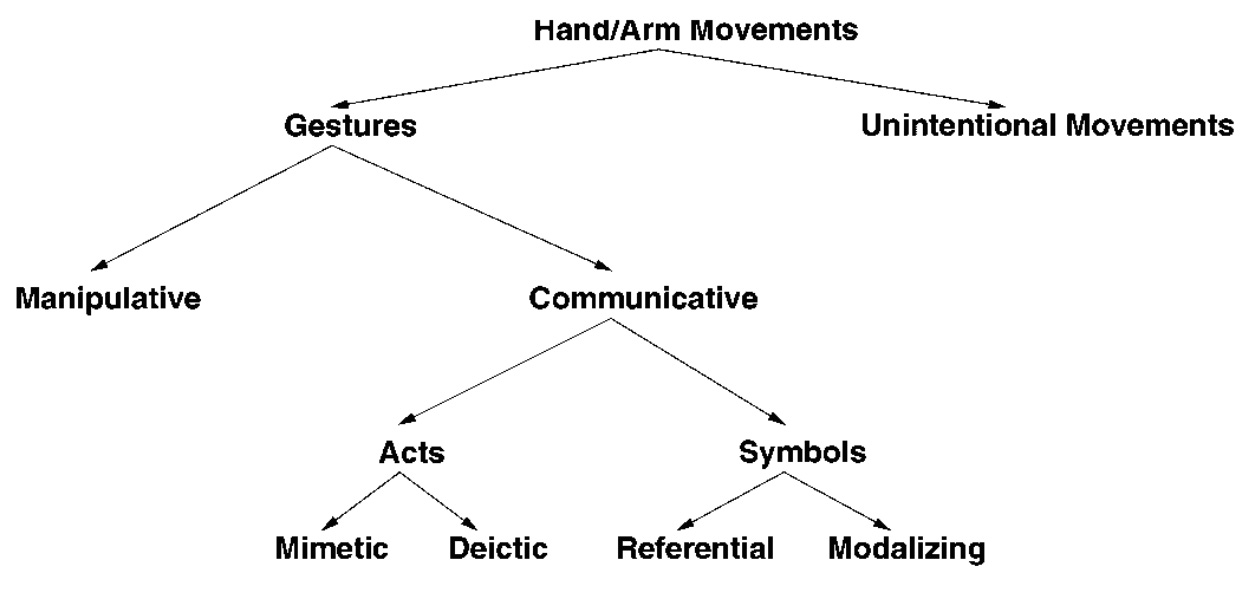
\includegraphics[width=120mm]{/content/ges-tax.jpg} \caption{The taxonomy of Hand Gestures. \cite{2}} \label{fg:ges:tax} 
\end{figure}


Manipulative gestures are the ones used to act on objects. For example, moving a chair from one location to another. Manipulative gestures in the context of HRI are mainly developed for medical surgery. Communicative gestures, on the other hand, have purely communicational purpose. In a natural environment they are usually accompanied by speech or spoken as a sign language. In HRI context these gesture are one of the commonly used gestures, since they can often be represented by static as well as dynamic hand postures.

In this thesis, we focus on communicative gestures in the form of symbols. They symbolize some referential action. For instance, circular motion of hand may be referred as an alphabet "O" or as an object such as wheel or as a command to turn in a circular motion.

\subsection{Feature Extraction} Feature extraction stage is concerned with the detection of features which are used for the estimation of parameters of the chosen gestural model. In the detection process it is first necessary to localize the user. 

\subsubsection{OpenNI 2} OpenNI or Open Natural Interaction is a framework by the company PrimeSense and open source software project focused on certifying and improving interoperability of natural user interfaces and organic user interfaces for Natural Interaction (NI) devices, applications that use those devices and middleware that facilitates access and use of such devices. Microsoft Kinect and Asus Xtion are commercially available depth cameras which are compatible with OpenNI.

The OpenNI 2.0 API provides access to PrimeSense compatible depth sensors. It allows an application to initialize a sensor and receive depth, RGB, and IR video streams from the device. OpenNI also provides a uniform interface that third party middleware developers can use to interact with depth sensors. Applications are then able to make use of both the third party middleware, as well as underlying basic depth and video data provided directly by OpenNI.

C++ code \ref{code:ni:device} shows how a depth camera such as Asus Xtion Pro can be used to retrieve depth information using OpenNI 2 framework.

\lstinputlisting[language=c++]{code/openni.cpp} \label{code:ni:device}

\subsubsection{NiTE 2} \label{sec:nite} PrimeSense's Natural Interaction Technology for End-user is the middleware that perceives the world in 3D, based on the PrimeSensor depth images, and translates these perceptions into meaningful data in the same way that people do. NITE middleware includes computer vision algorithms that enable identifying users and tracking their movements. Figure shows the architecture of NiTE, how it is working together with OpenNI, depth sensors and applications.

Figure \ref{fg:ni:arch} displays a layered view of producing, acquiring and processing depth data, up to the level of the application that utilizes it to form a natural- interaction based module. 

\begin{figure}
	[h] \centering 
	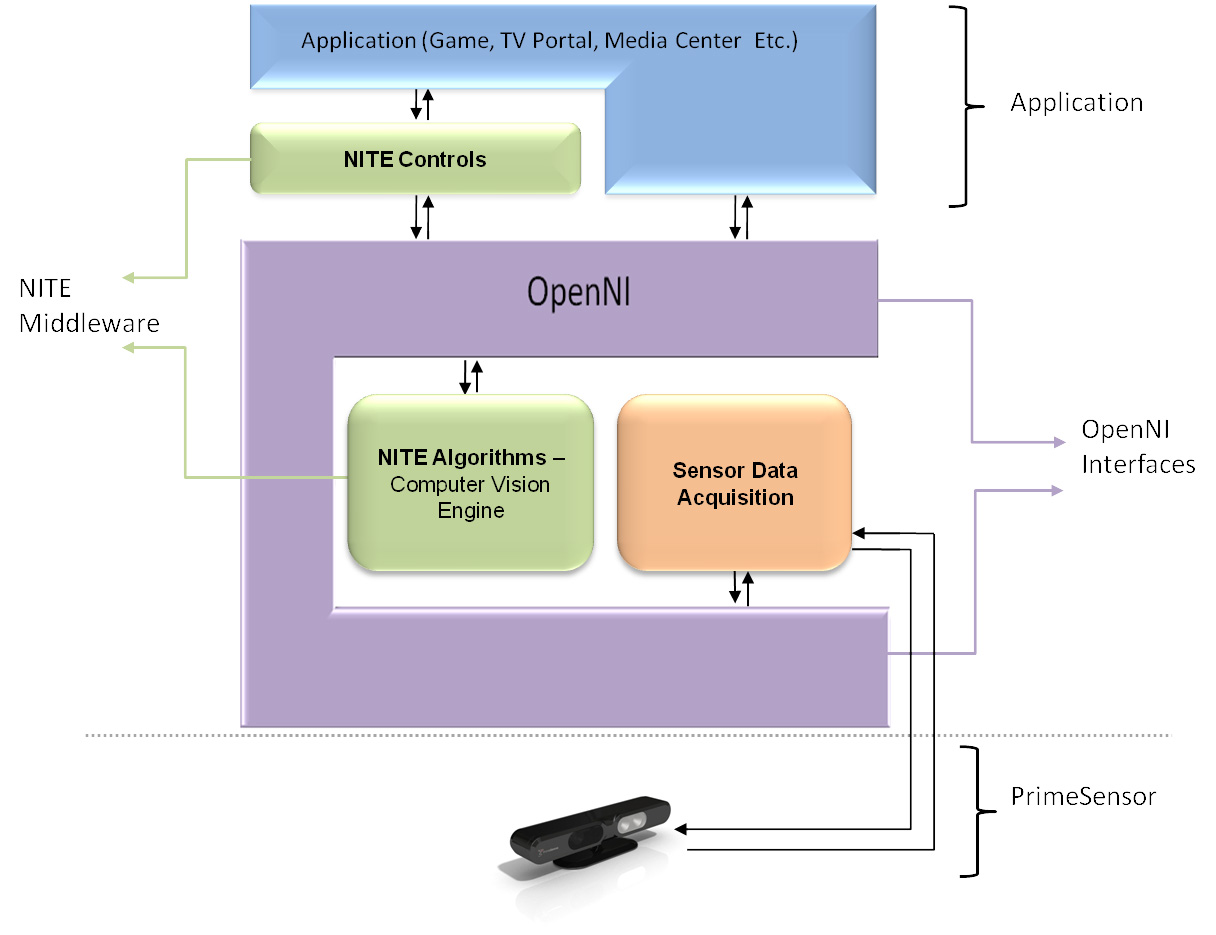
\includegraphics[height=10cm]{figures/content/ni-arch.jpg} \caption{NiTE Architecture} \label{fg:ni:arch} 
\end{figure}

\begin{itemize}
	\item The lower layer is the PrimeSensor device, which is the physical acquisition layer, resulting in raw sensory data from a stream of depth images. 
	\item The next Cshaped layer is executed on the host PC represents OpenNI. OpenNI provides communication interfaces that interact with both the sensor's driver and the middleware components, which analyze the data from the sensor. 
	\item The sensor data acquisition is a simple acquisition API, enabling the host to operate the sensor. This module is OpenNI compliant interfaces that conforms to OpenNI API standard. 
	\item The NITE Algorithms layer is the computer vision middleware and is also plugged into OpenNI. It processes the depth images produced by the PrimeSensor. 
	\item The NITE Controls layer is an applicative layer that provides application framework for gesture identification and gesture-based UI controls, on top of the data that was processed by NITE Algorithms. 
\end{itemize}

\subsubsection{Skeletal Points Tracking Algorithm} The lower layer of NiTE middleware that performs the groundwork of processing the stream of raw depth images. This layer utilizes computer vision algorithms to perform the following: 
\begin{itemize}
	\item Scene segmentation is a process in which individual users and objects are separated from the background and tagged accordingly. 
	\item Hand point detection and tracking 
	\item Full body tracking based on the scene segmentation output. Users bodies are tracked to output the current user pose a set of locations of body joints. 
\end{itemize}

NiTE uses machine learning algorithms to recognize anatomical landmarks and pose of human body \cite{}. Figure \ref{fg:ni:alg} shows how NiTE tracks human skeleton from a single input depth image and a per-pixel body part distribution is inferred. Colors indicate the most likely part labels at each pixel and correspond to the joint proposals. Local modes of this signal are estimated to give high-quality proposals for the 3D locations of body joints, even for multiple users.

\begin{figure}
	[h] \centering 
	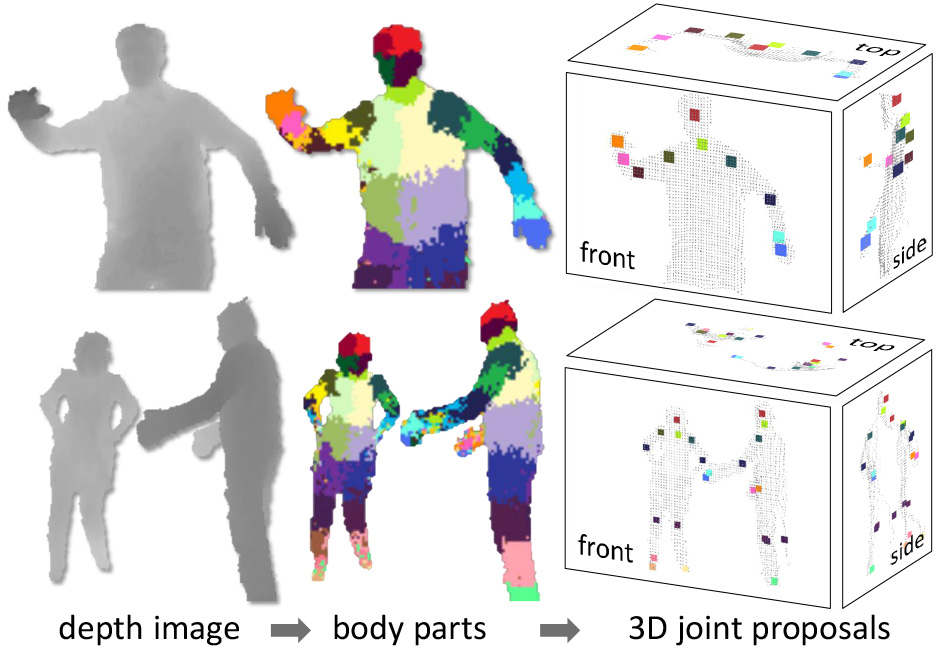
\includegraphics[height=8cm]{/content/ni-alg.jpg} \caption{Skeleton Tracking algorithm processes a depth image and a per-pixel body part distribution is inferred, and finally, 3D joints proposals are made for 15 points in human skeleton. \cite{13} } \label{fg:ni:alg} 
\end{figure}


\paragraph*{Training} In order to train the system, large collection of synthetic and real representations of human body were recorded and labeled. Each body representations was covered with several localized body part labels as show in the figure \ref{fg:ni:train}. Some of these parts are defined to directly localize particular skeletal joints of interest, while others fill the gaps or could be used in combination to predict other joints.

\begin{figure}
	[h] \centering 
	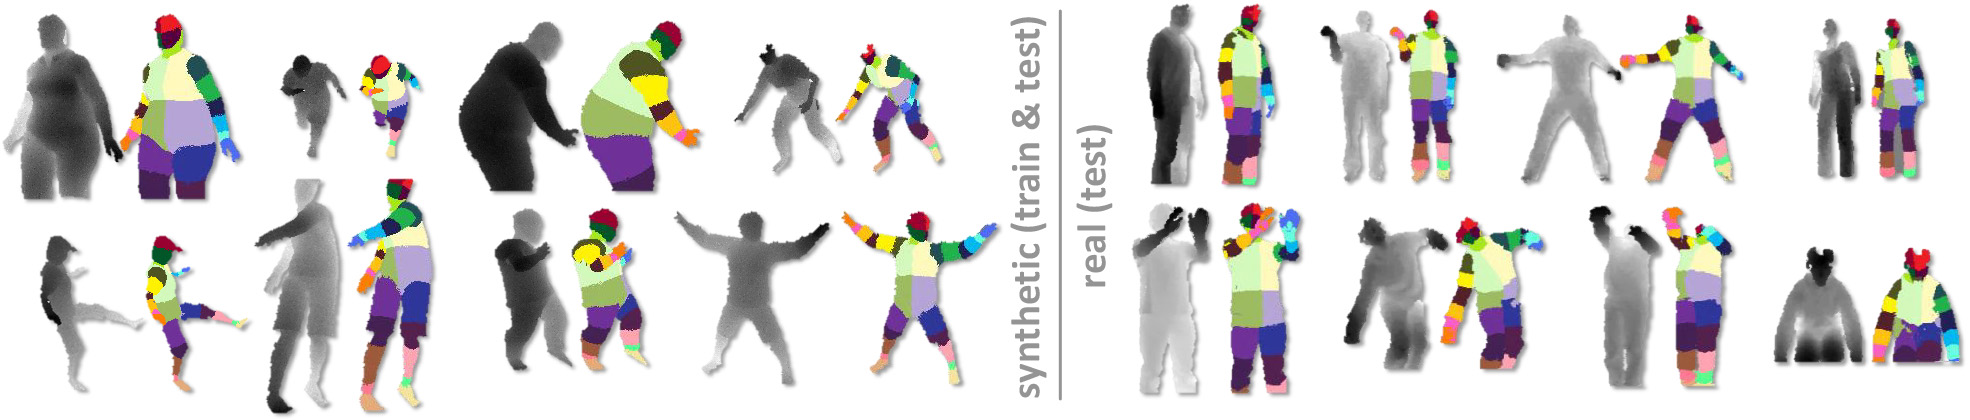
\includegraphics[height=3cm]{figures/content/ni-train.jpg} \caption{NiTE Synthetic and real training} \label{fg:ni:train} 
\end{figure}


\paragraph*{Feature Labeling} Features are located in depth image as shown in the figure \ref{fg:ni:label} and labeled. The yellow crosses indicates the pixel x being classified. The red circles indicate the offset pixel. In (a), the two example features give a large depth difference response. In (b), the same two features at new image locations give a much smaller response.

\begin{figure}
	[h] \centering 
	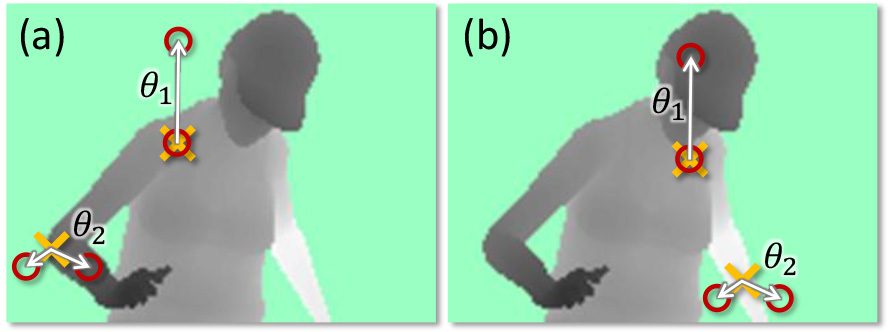
\includegraphics[height=4cm]{figures/content/ni-label.jpg} \caption{Features are located in depth image and labeled. \cite{2}} \label{fg:ni:label} 
\end{figure}


\paragraph*{Classification} Randomized decision forest is the classification algorithm used by NiTE to predict the probability of a pixel belonging to a body part. Randomized decision trees and forests have proven fast and effective multi-class classifiers for many tasks. Figure \ref{fg:ni:decision} shows Randomized Decision Forests. A forest is an ensemble of trees. Each tree consists of split nodes (blue) and leaf nodes (green). The red arrows indicate the different paths that might be taken by different trees for a particular input.

\begin{figure}
	[h] \centering 
	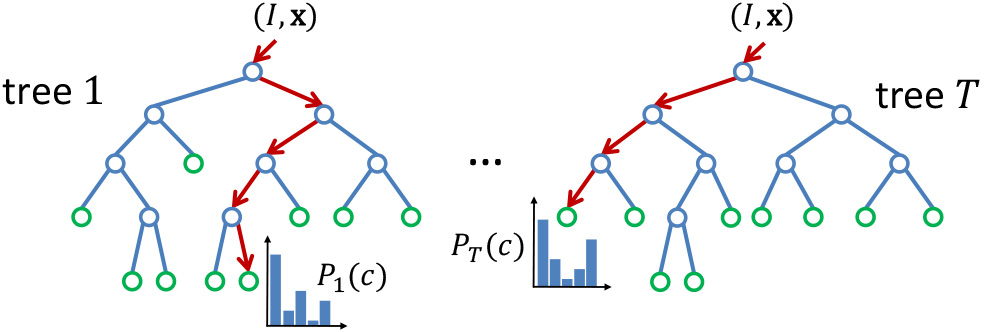
\includegraphics[height=4cm]{figures/content/ni-decision.jpg} \caption{Randomized decision forest} \label{fg:ni:decision} 
\end{figure}


\paragraph*{Prediction} To classify pixel x in image I using Randomized decision tree, one starts at the root and repeatedly evaluates equation \ref{eq:ni:decision}, branching left or right according to the comparison to threshold {$ \tau\ $}. At the leaf node reached in tree t, a learned distribution $ P_{t}(c|I,x) $ over body part labels c is stored. The distributions are averaged together for all trees in the forest to give the final classification.

\begin{equation}
\LARGE 
P_{t}(c|I,x) = \frac{1}{T} \sum_{t=1}^{T} P_{t}(c|I,x)
\label{eq:ni:decision}
\end{equation}

Each tree is trained on a different set of randomly synthesized images. A random subset of 2000 example pixels from each image is chosen to ensure a roughly even distribution across body parts. Training phase was conducted in distributed manner by training 3 trees from 1 million images on 1000 core cluster.

After predicted the probability of a pixel belonging to a body part, the body parts are recognized and reliable proposals for the positions of 3D skeletal joints are generated. These proposals are the final output of the algorithm and used by a tracking algorithm to self initialize and recover from failure.

\begin{figure}
	[h] \hspace{-5 mm} 
	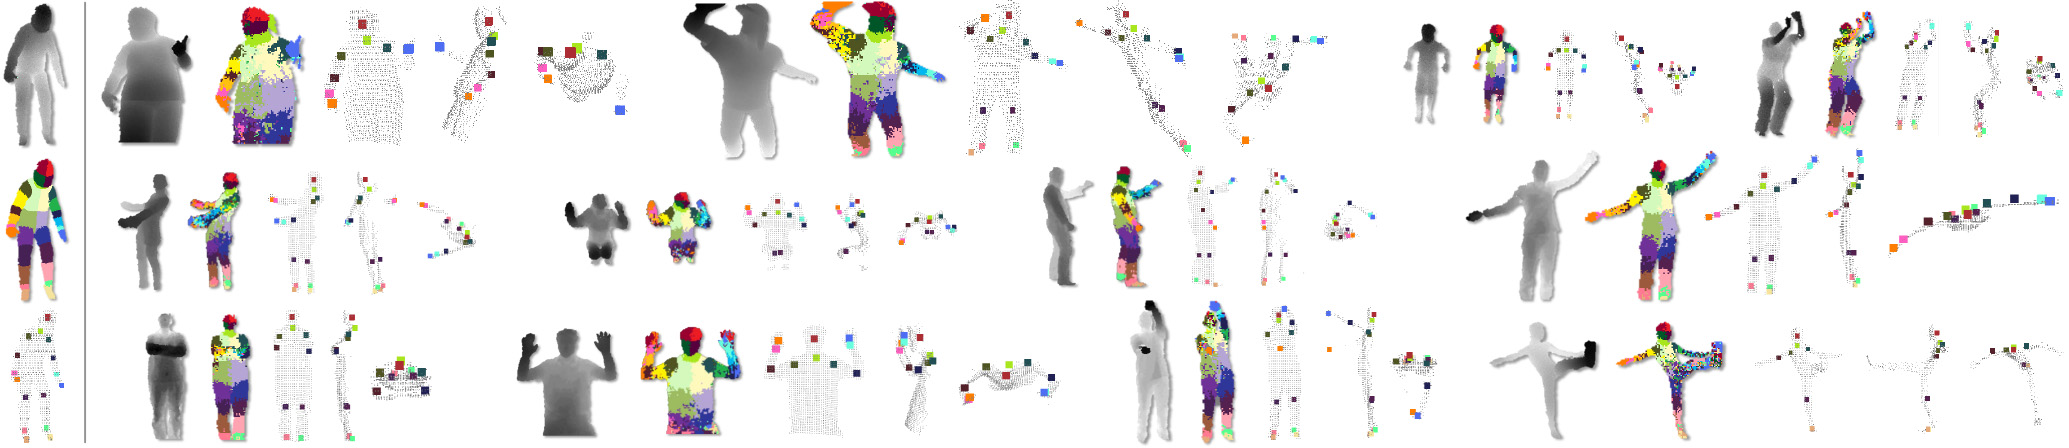
\includegraphics[width=160mm]{figures/content/ni-pose.jpg} \caption{Joint proposals are derived for various poses. Results of synthetic training data is shown on the top row, real training data shown in the middle row and failure modes at bottom. Left column shows a neutral pose as a reference. \cite{13} } \label{fg:ni:pose} 
\end{figure}


\paragraph*{Joints Proposal} Figure \ref{fg:ni:pose} shows example inferences. Synthetic (top row); real (middle); failure modes (bottom). Left column: ground truth for a neutral pose as a reference. In each example we see the depth image, the inferred most likely body part labels, and the joint proposals show as front, right, and top views (overlaid on a depth point cloud). Only the most confident proposal for each joint above a fixed, shared threshold is shown.

\paragraph*{Skeletal points} Finally NiTE API returns positions and orientations of the skeleton joints as shown in the figure \ref{fg:ni:joints}. As well as it returns the lengths of the body segments such as the distance between returned elbow and shoulder. Joint positions and orientations are given in the real world coordinate system. The origin of the system is at the sensor. +X points to the right of the, +Y points up, and +Z points in the direction of increasing depth. 

\begin{figure}
	[h]
	\centering
	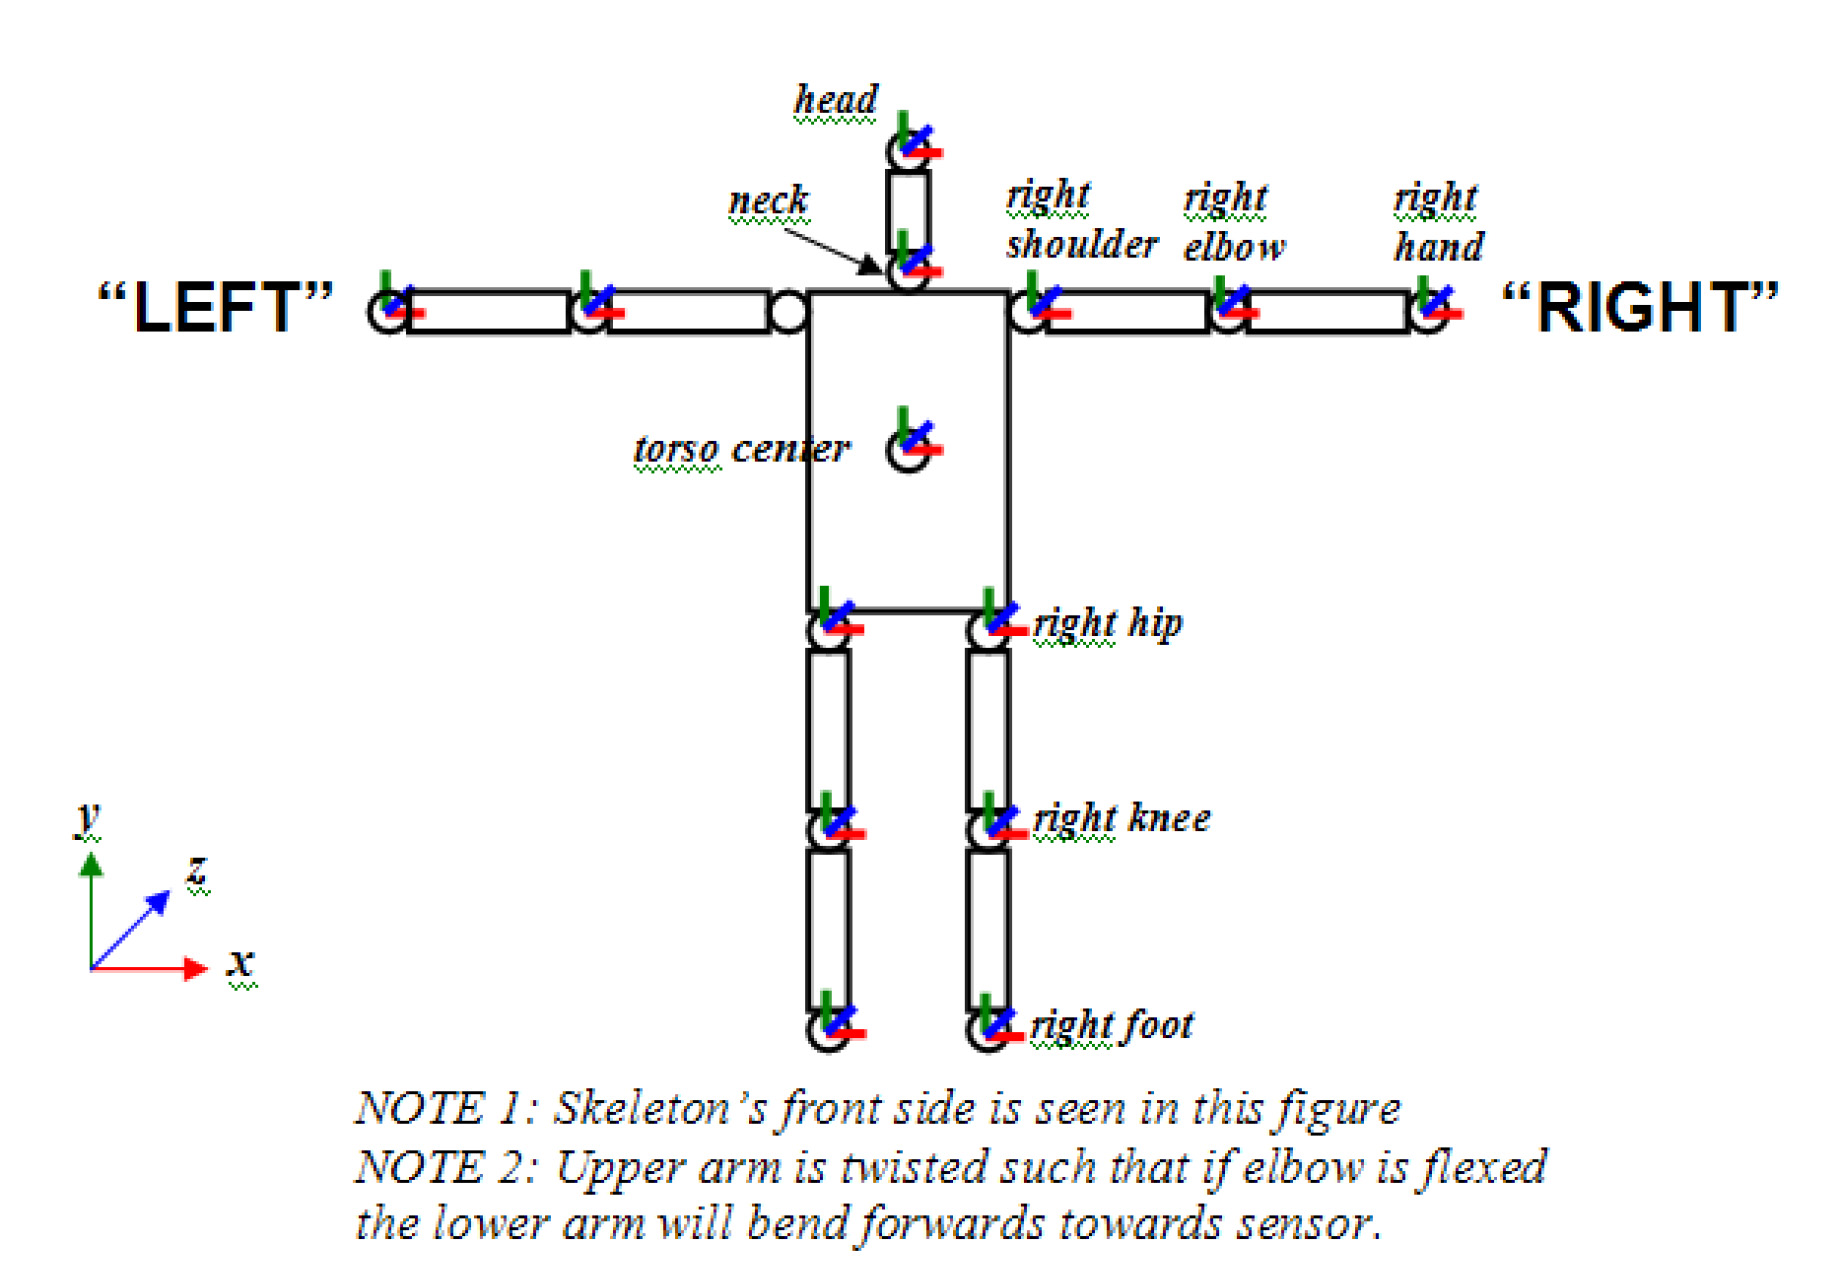
\includegraphics[height=10cm]{/content/ni-joints.jpg} \caption{Positions and orientations of the tracked skeleton return by NiTE API. \cite{12}} \label{fg:ni:joints} 
\end{figure}


\paragraph*{Hand Tracker} Even though NiTE framework can recognize full human body, in this thesis we have used only hand recognition and tracking due to computational limitation of NAO. NiTE provides an interface track only a hand in real time. In order to start tracking a hand, a focus gesture must be gesticulated. There are two supported focus gestures: click and wave. In the click gesture, you should hold your hand up, push your hand towards the sensor, and then immediately pull your hand back towards you. In the wave gesture, you should hold your hand up and move it several times from left to right and back. Once hand is been found and it will be tracked till the hand leaves the field of view of the camera or hand point is lost due to various factors such as hand was touching another object or closer to another body part. Figure \ref{fg:ni:hand} shows how hand points are tracked using NiTE and trail of the hand positions in real world coordinates are mapped on to the depth image.

\begin{figure}
	\centering 
	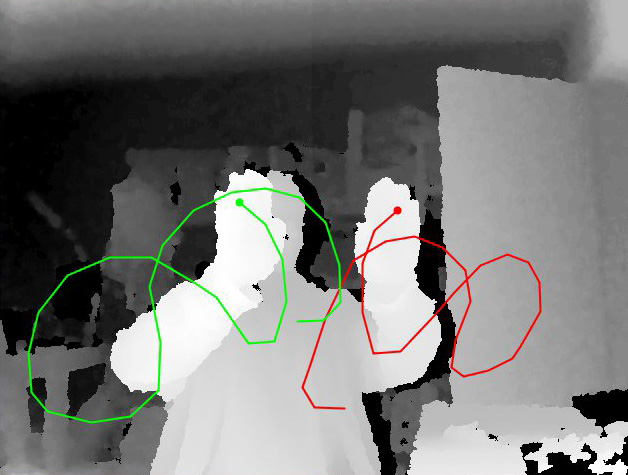
\includegraphics[height=8cm]{/content/ni-hand.jpg} \caption{NiTE Hand Tracking application shows the trail of the tracked hand in different colors. \cite{12} } \label{fg:ni:hand} 
\end{figure}


\paragraph*{Focus gestures} Focus gestures of NiTE is can be detected even after initiating the hand tracking. NITE gestures are derived from a stream of hand points which record how a hand moves through space over time. Each hand point is the real-world 3D coordinate of the center of the hand, measured in millimeters. Gesture detectors are sometimes called point listeners (or point controls) since they analyze the points stream looking for a gesture. 

NiTE recommends user to follow these suggestions to gain maximum efficiency from its API. 
\begin{itemize}
	\item Try to keep the hand that performs the gesture at a distance from your body. 
	\item Your palm should be open, fingers pointing up, and face the sensor. 
	\item The movement should not be too slow or too fast. 
	\item WAVE movement should consist of at least 5 horizontal movements (left-right or right-left) 
	\item CLICK movement should be long enough (at least 20 cm). 
	\item Make sure CLICK gesture is performed towards the sensor. 
	\item If you have difficulty to gain focus, try to stand closer to the sensor (around 2m), and make sure that your hand is inside the field of view. 
\end{itemize}

Finally, C++ code \ref{code:ni:nite} shows shows how hand tracking can be initiated using a focus gesture. 

\lstinputlisting[language=c++]{code/nite.cpp} \label{code:ni:nite}

\subsection{Gesture Classification and Prediction} Like most other recognitions such as speech recognition and biometrics, the tasks of gesture recognition involve modeling, feature extraction, training, classification and prediction as shown in the figure \ref{fg:grt:pipeline}. Though the alternatives such as Dynamic Programming (DP) matching algorithms have been attempted, the most successful solutions involves feature-based statistical learning algorithm. Previous sections explained how gesture is modelled and feature is extracted from raw depth images, and the following sections discuss how extracted feature inputs are trained, classified and predicted.

In this thesis, we have chosen a machine learning technique based on Adaptive Naive Bayes Classifier (ANBC) with the help of Gesture Recognition Toolkit. ANBC is an extension to the well-known Naive Bayes, one of the most commonly used supervised learning algorithms that works very well on both basic and more complex recognition problems.

\subsubsection{Adaptive Naive Bayes Classifier} \label{sec:anbc} ANBC \cite{14} is a supervised learning algorithm that can be used to classify any type of N-dimensional signal. It is based on simple probabilistic classifier called Naive Bayes classifier. It fundamentally works by fitting an N-dimensional Gaussian distribution to each class during the training phase. New gestures can then be recognized in the prediction phase by finding the gesture that results.

ANBC like Naive Bayes classifier makes a number of basic assumptions with input data that all the variables in the data are independent. However, despite these naive assumptions, Naive Bayes Classifiers have proved successful in many real-world classification problems \cite{15}. It has also been shown in a study that the Naive Bayes Classifier not only performs well with completely independent features, but also with functionally dependent features.

ANBC algorithm is based on Bayes theory and gives the likelihood of event $A$ occurring, given the observation of event $B$. In the equation \ref{eq:grt:bayes}, $P(A)$ represents the prior probability of event $A$ occurring and $P(B)$ is a normalizing factor to ensure that all the posterior probabilities sum to 1.

\begin{equation}
P(A|B) = \frac{P(B|A) P(A)}{P(B)}
\label{eq:grt:bayes}
\end{equation}

\paragraph*{Training} The weighting coefficient adds an important feature for the ANBC algorithm as it enables one general classifier to be trained with multidimensional inputs, even if a number of inputs are only relevant for one particular gesture. For example, if it is used to recognize hand gestures, the weighting coefficients would enable the classifier to recognize both left and right hand gestures independently, without the position of the left hand affecting the classification of a right-handed gesture. For example, hand gesture recognition using x,y,z position of palms of Left and Right hand will have 6 dimensional sample. In this case left hand gestures will have weights {1,1,1,0,0,0}, right hand gestures will have weights {0,0,0,1,1,1} and both hand gestures will have weights {1,1,1,1,1,1}.

Using the weighted Gaussian model, the ANBC algorithm requires $G(3N)$ parameters, assuming that each of the $G$ gestures require specific values for the N-dimensional $ \mu_{k} , \sigma_{k}^{2} $ and $ \phi_{k} $ vectors where $ \mu_{k} , \sigma_{k}^{2},\phi_{k}$ are mean, variance and weighting coefficients. Assuming that $ \phi_{k} $ is set by the user, $ \mu_{k} $ and $\sigma_{k}^{2} $ values can easily be calculated in a supervised learning scenario by grouping the input training data $X$ into a matrix containing $M$ training examples each with $N$ dimensions, into their corresponding classes. The values for $ \mu$ and $\sigma^{2} $of each dimension $n$ for each class $k$ can then be estimated by computing the mean and variance of the grouped training data for each of the respective classes \cite{14}.

\begin{equation}
P(g_{k}|x) = \frac{P(x|g_{k}) P(g_{k})} {\sum_{i=1}^{G}P(x|g_{i}) P(g_{i})} \:\:\:\:\: 1\leq k \leq G
\label{eq:grt:gauss}
\end{equation}

After the Gaussian models have been trained for each of the $G$ classes, an unknown N-dimensional vector $x$ can be classified as one of the $G$ classes using the maximum a posterior probability estimate (MAP). MAP estimate classifies $x$ as the $k$-th class that results in the maximum a posterior probability given by the equation \ref{eq:grt:gauss}

\begin{equation}
ln N (x|\Phi_{k}) \:\:\:\:\: 1\leq k \leq G
\label{eq:grt:threshold}
\end{equation}

\paragraph*{Rejection Threshold} Using equation \ref{eq:grt:threshold}, an unknown N-dimensional vector $x$ can be classified as one of the $G$ classes from a trained ANBC model. If $x$ actually comes from an unknown distribution that has not been modeled by one of the trained classes then, it will be incorrectly classified against the $k$ th gesture that gives the maximum likelihood value. A rejection threshold must therefore be calculated for each of the $G$ gestures to enable the algorithm to classify any of the $G$ gestures from a continuous stream of data that also contains non-gestural data \cite{14}.

\paragraph*{Online Training} One key element of ANBC is that it can easily be made adaptive. Adding an adaptive online training phase to the common two-phase (training and prediction) provides some significant advantages for the recognition gestures. During online training phase the algorithm will not only perform real-time predictions on the continuous stream of input data, but it will also continue to train and refine the models for each gesture. This enables the user to initially train the algorithm with a low number of training samples and during the adaptive online training phase, the algorithm can continue to train and refine the initial models, creating a more robust model as the number of training samples increases.

\paragraph*{Pros / Cons} ANBC works well for the classification of static gestures and non-temporal pattern recognition. However, the main limitation of the ANBC is that, it does not work well when the data you want to classify, is not linearly separable because it uses a Gaussian distribution to represent each class. Also when ANBC is working with online training enabled, a small number of incorrectly labeled training examples can create a loose model that becomes less effective at each update step and ultimately lead to a poor performance and accuracy.

\subsubsection{Gesture Recognition Toolkit (GRT)} \label{sec:grt} GRT is a cross-platform open-source C++ library designed and developed mainly by Nicholas Gillian at MIT Media Lab to make real-time machine learning and gesture recognition \cite{16}. Emphasis is placed on the ease of use with a consistent, minimalist design that promotes accessibility while supporting flexibility and customization for advanced users. The toolkit features a broad range of classification and regression algorithms, and has extensive support for building real-time systems. GRT includes algorithms for signal processing, feature extraction and automatic gesture spotting. 

In this thesis, we attempt to take advantage of GRT as framework to carry out most of the tasks involved in hand gesture recognition. Figure \ref{fg:grt:pipeline} shows that GRT provides the full fledge pipeline to build a real-time gesture recognition system. 

\begin{figure}
	[h] \hspace{-5 mm} 
	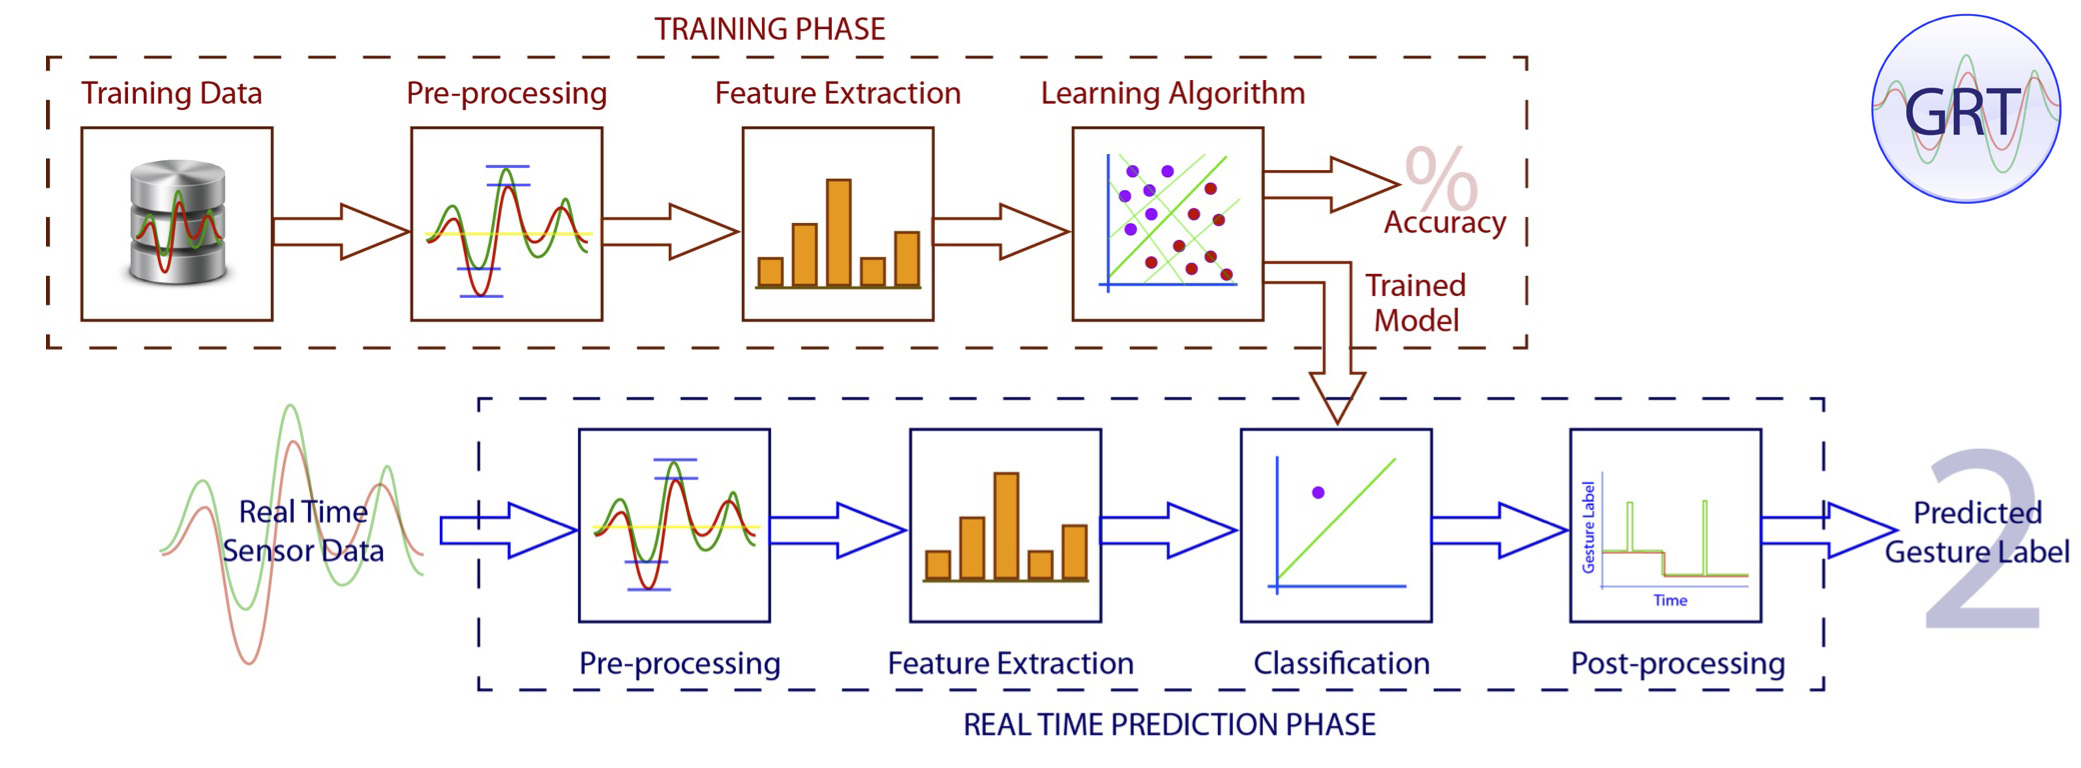
\includegraphics[width=160mm]{figures/content/grt-pipeline.jpg} \caption{Stages of Gesture Recognition which are supported by GRT Recognition Pipeline. \cite{16} } \label{fg:grt:pipeline} 
\end{figure}


\paragraph*{Pipeline} GRT provides an API to reduce the need for boilerplate code to perform common functionality, such as passing data between algorithms or to per-process data sets. GRT uses an object-oriented modular architecture and it is built around a set of core modules and a gesture-recognition pipeline. The input to both the modules and pipeline consists of an N-dimensional double-precision vector, making the toolkit flexible to any type of input signal. The algorithms can be used as stand-alone classes; alternatively a gesture recognition pipeline can be used to chain modules together to create a more sophisticated gesture recognition system. Modularity of GRT pipeline offers developers opportunities to work on each stages of gesture recognition independently. Additionally, pipeline can be stored and loaded dynamically so that an compiled application can work in many different configurations. 

\paragraph*{ClassificationData} Accurate labeling of dataset is very critical for machine learning problems. The toolkit thus contains an extensive support for recording, labeling and managing supervised and unsupervised datasets for classification, regression and time series analysis. \textit{ClassificationData} is the data structure used for supervised learning problems and for most of the non temporal classification algorithms.

GRT allows us to store and load the training data in GRT format or Comma Separated Values (CSV). Since the training datasets are stored in human readable format, it enables us to add more samples which are collected separately or remove false data from the training dataset.

\paragraph*{TrainingDataRecordingTimer} Important part of the training phase is recording positive samples of modeled hand gestures. Hence, GRT provides a feature called \textit{TrainingDataRecordingTimer} that sets recording and preparation time in milliseconds. Once it is started by calling \textit{startRecording(prepationTime, recordTime)} method, it waits for given preparation time before it actually starts to store the data. This feature helps the trainer get into the right pose before samples are added to the training data and as well as train all the gestures for the same time duration.

\paragraph*{Algorithms} GRT features a broad range of machine-learning algorithms such as AdaBoost, Decision Trees, Dynamic Time Warping (DTW), Hidden Markov Models (HMM), K-Nearest Neighbor (KNN), Linear and Logistic Regression, Adaptive Naive Bayes (ANBC), Multilayer Perceptrons (MLP), Random Forests and Support Vector Machines (SVM) \cite{16}. 

\paragraph*{Null Rejection} Another important feature of GRT is Null Rejections threshold. It means that algorithms can automatically spot the difference between trained gestures and unintended gestures that can happen when the user moves the hand in freely. It can be enabled by the method \textit{enableNullRejection(true)} and the range of the null rejection region can be set by this method \textit{setNullRejectionCoeff(double nullRejectionCoeff)} of the classifier. Algorithm such as the ANBC and N-Dimensional DTW, learn rejection thresholds from the training data, which are then used to automatically recognize valid gestures from a continuous stream of real-time data.

\begin{figure}
	[h] \centering 
	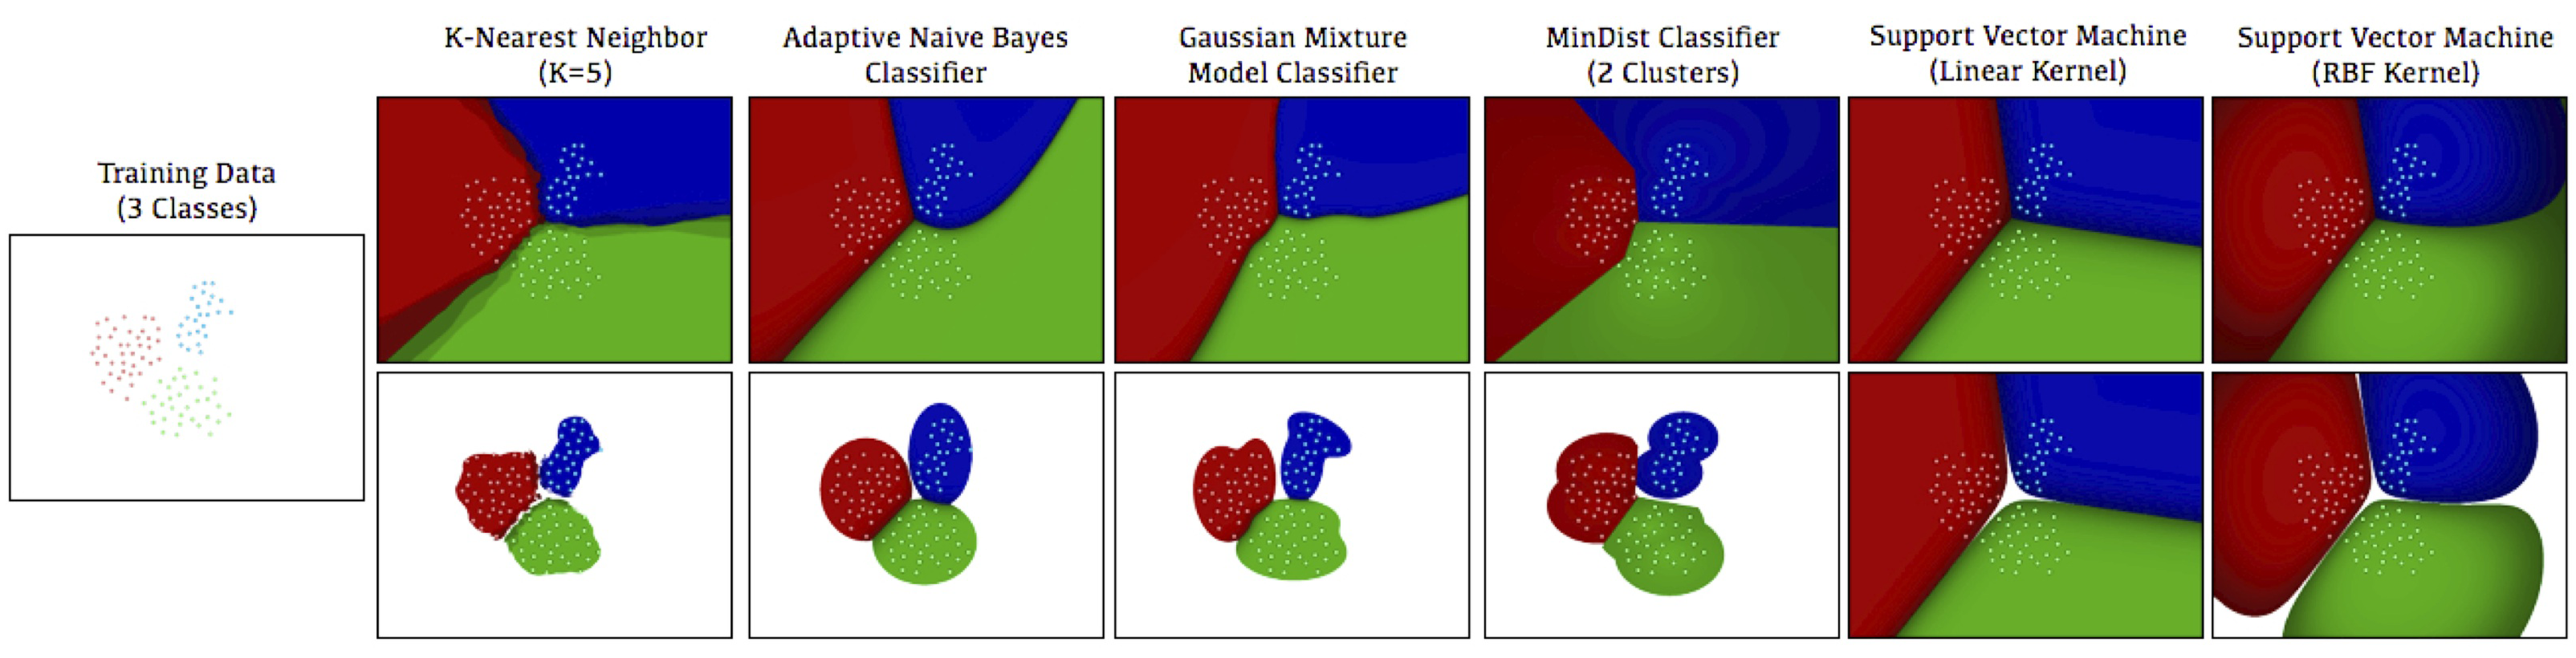
\includegraphics[height=35mm]{figures/content/grt-null.png} \caption{GRT Null Rejection} \label{fg:grt:null} 
\end{figure}


Figure \ref{fg:grt:null} shows that the decision boundaries computed by training six of classification algorithms on an example dataset with 3 classes. After training each classifier, each point in the two-dimensional feature space is colored by the likelihood of the predicted class label (red for class 1, green for class 2, blue for class 3). The top row shows the predictions of each classifier with null rejection disabled. The bottom row shows the predictions of each classifier with null rejection enabled with a coefficient of 3.0. Rejected points are colored white. Note that both the decision boundaries and null-rejection regions are different for each of the classifiers. This results from the several learning and prediction algorithms used by each classifier. 

\paragraph*{Scaling Normalization} Real-time classification faces normalization problems when the range of training data differ from prediction input. To solve this problems, there are few solutions such as Z-score Standardization and Feature Scaling. GRT presents a simple solution called as Minimum-Maximum scaling.

Min-Max scaling rescales the range in [0, 1] or [-1, 1]. Selecting the target range depends on the nature of the data. Classifiers \textit{enableScaling(true)} method scales input vector between the default min-max range that is from 0 to 1. The cost of having this bounded range is that model will end up with smaller standard deviations, which can suppress the effect of outliers. Equation \ref{eq:grt:scaling} shows how Min-Max scaling is done.

\begin{equation}
\large 
x{}' = \frac{x - min(x)}{max(x) - min(x)}
\label{eq:grt:scaling}
\end{equation}

\paragraph*{Pre/Post Processing Modules} In many real-world scenarios, the input to a classification algorithm must be preprocessed and have salient features extracted. GRT therefore supports a wide range of pre/post-processing modules such as Moving Average Filter, Class Label Filter and Class Label Change Filter, embedded feature extraction algorithms such as AdaBoost, dimensionality reduction techniques such as Principal Component Analysis (PCA) and unsupervised quantizers such as K-Means Quantizer, Self-Organizing Map Quantizer.

There will not be any need of preprocessing modules in this project since raw data received from depth sensor is processed by NiTE framework. However, post-processing modules such as Class Label Filter and Class Label Change Filter may be needed for a reasons that depth sensor samples 30 frames per second, therefore 30 input samples per second are supplied to the classifier for prediction and the output must be triggered once for every gesture. 

\begin{figure}
	[h] \centering 
	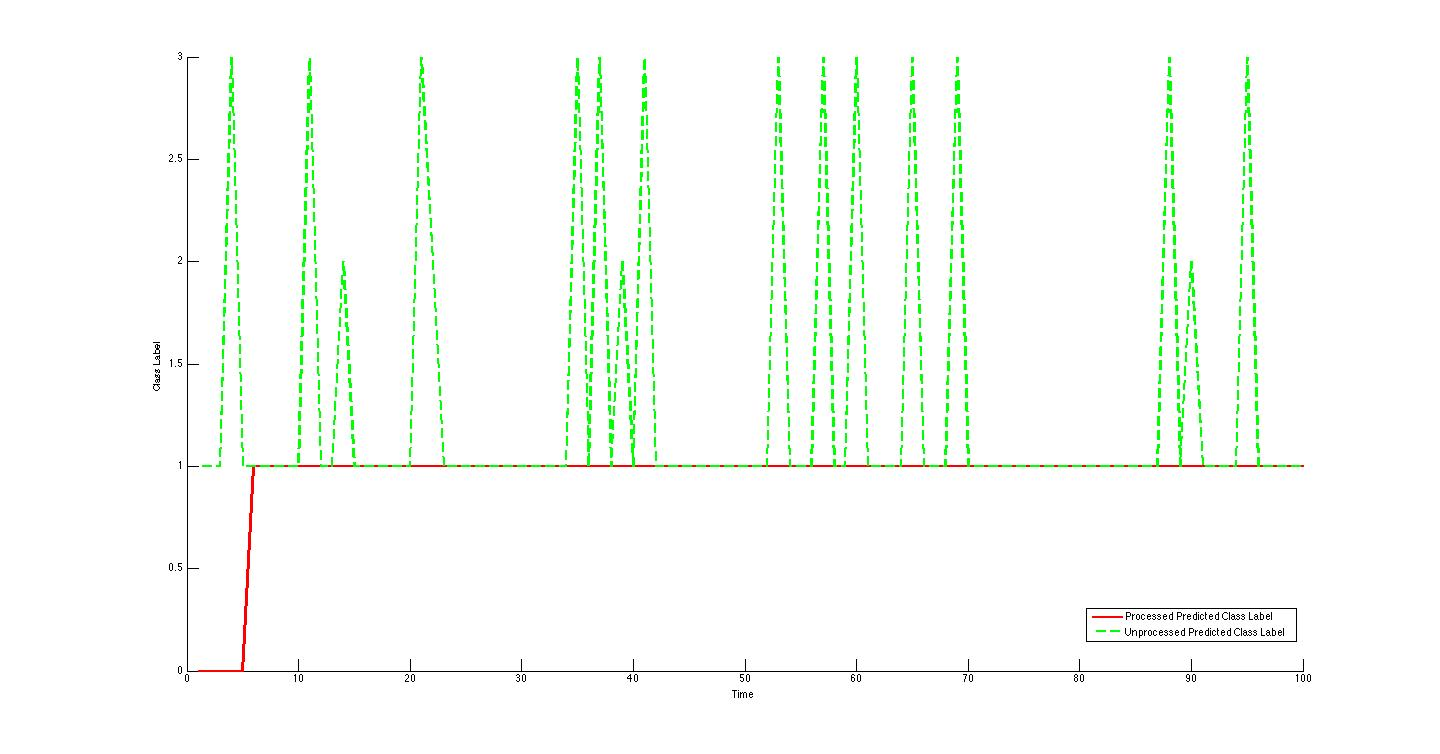
\includegraphics[height=7cm]{/content/grt-label-filter.jpg} \caption{GRT Class Label Filter removes the sporadic prediction values and outputs buffered class label. \cite{16}} \label{fg:grt:label} 
\end{figure}


\paragraph*{Class Label Filter} It is a useful post-processing module which can remove erroneous or sporadic prediction spikes that may be made by a classifier on a continuous input stream of data. Figure \ref{fg:grt:label} that the classifier correctly outputs the predicted class label of 1 for a large majority of the time that a user is performing gesture 1. However, may be due to sensor noise or false samples in the training data, the classifier outputs the class label of 2. In this instance the class label filter can be used to remove these sporadic prediction values with the output of the class label filter in this instance being 1. 

Class Label Filter module is controlled through two parameters: the minimum count value and buffer size value. The minimum count sets the minimum number of label values that must be present in the buffer to be output by the Class Label Filter. The size of the class labels buffer is set by the buffer size parameter. If there is more than one type of class label in the buffer then the class label with the maximum number of instances will be output. If the maximum number of instances for any class label in the buffer is less than the minimum count parameter then the Class Label Filter will output the default null rejection class label of 0.

\begin{figure}
	[h] \centering 
	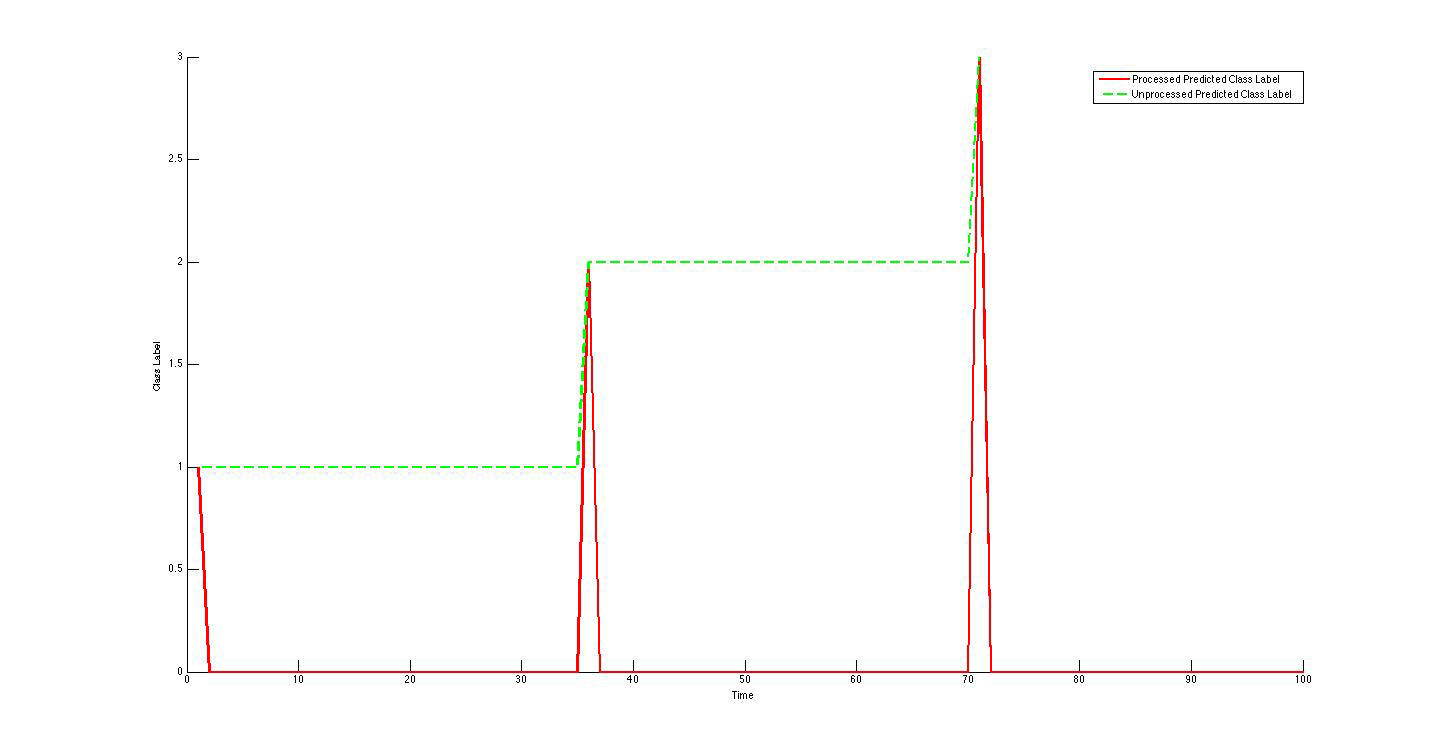
\includegraphics[height=7cm]{figures/content/grt-label-change-filter.jpg} \caption{GRT Label Change Filter outputs only when there is change in the prediction. \cite{16}} \label{fg:grt:label:change} 
\end{figure}


\paragraph*{Class Label Change Filter} It is one of the useful post-processing module that triggers when the predicted output of a classifier changes. Figure \ref{fg:grt:label:change}shows that, if the output stream of a classifier is {1,1,1,1,2,2,2,2,3,3}, then the output of the filter would be {1,0,0,0,2,0,0,0,3,0}. This module is useful to trigger a gesture once, if the user is gesticulating the same gesture for longer time duration. If the user intends to trigger the same gesture again, then hand position must be changed to another such as pointing the hand towards the ground, and gesticulate the gesture again.

\paragraph*{GUI} Figure \ref{fg:grt:gui} shows GRT-GUI which is an application that provides an easy-to-use graphical interface developed in C++ to setup and configure a gesture recognition pipeline that can be used for classification, regression, or time-series analysis. Data and control commands are streamed in and out of this application as Open Sound Control (OSC) packets via UDP . Therefore, it acts as a standalone application to record, label, save, load and test the training data and performs a real-time prediction for the incoming data, send output to another application. 

\begin{figure}
	[h] \centering 
	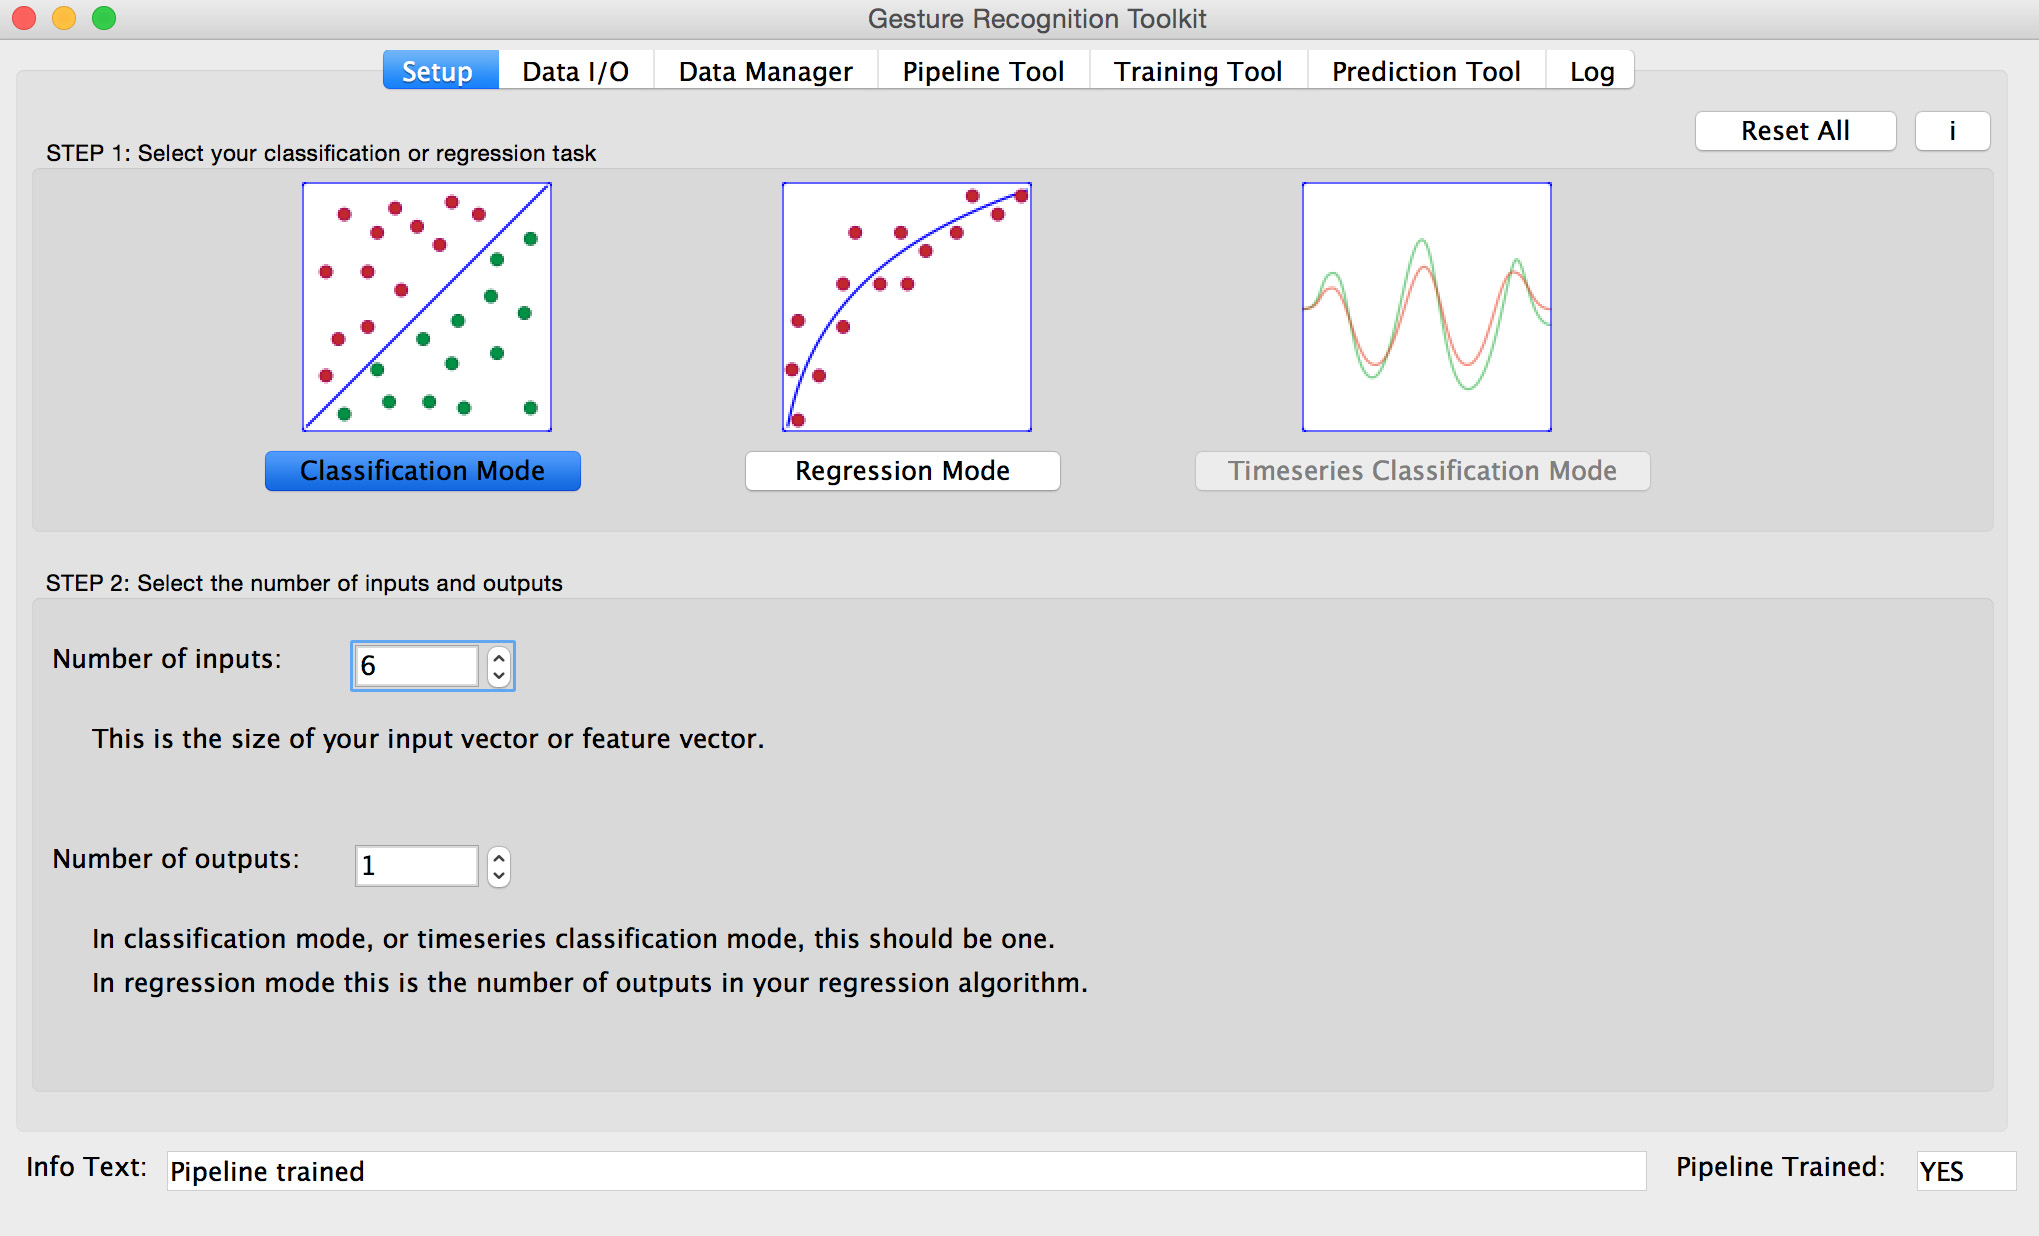
\includegraphics[height=7cm]{figures/content/grt-gui.jpg} \caption{GRT GUI is an standalone application to quick prototype by recording, labeling, saving, loading, testing the training data and to perform a real-time prediction. \cite{grt-spec}} \label{fg:grt:gui} 
\end{figure}
 
 


\section{Summary} This chapter has discussed the concepts of hand gesture recognition using skeletal points tracking with the help of depth camera. It has also talked about the specifications of Aldebaran NAO. Furthermore, It has discussed the features of the machine learning tool GRT that helps us to carry out the classification and prediction of hand gestures in real time.
